\documentclass[a4paper,10pt]{article}
\usepackage[utf8]{inputenc} %Codificacion utf-8
\usepackage{graphicx}
\usepackage{enumerate}
\usepackage{fancyhdr}
\usepackage{hyperref}
\usepackage{multirow} % Required for multirows
\usepackage[spanish, activeacute]{babel} %Definir idioma español
% \usepackage[margin=3cm]{geometry}
\hypersetup{
    colorlinks=true,
    linkcolor=black,
    filecolor=magenta,
    urlcolor=cyan,
}
\pagestyle{fancy}

\lhead{Análisis clínicos III}
\rfoot{Página \thepage}
\lfoot{Diego Rodríguez Riera}
\cfoot{Bases de Datos}
\newcommand\tab[1][1cm]{\hspace*{#1}}

\title{Análisis clínicos III\\{\small Revisión 3}}
\author{Diego Rodríguez Riera}
\date{\today}

\begin{document}

\maketitle
\pagebreak
\tableofcontents
\pagebreak

\section{Definición del problema.}
\paragraph{}
A lo largo de las clases impartidas el alumnado ha comprendido la importancia de una descripción rigurosa del problema del mundo real co n el fin de poder construir un modelo conceptual del mismo que sirva de base para la representación lógica del problema y su tratamiento mediante la tecnología de bases de datos.
\paragraph{}
Por lo tanto, como paso previo al uso de un modelo de datos para la construcción del modelo conceptual, es necesario llevar a cabo el estudio exhaustivo del problema planteado (Gestión de Análisis Clínicos).
\paragraph{}
En este estudio se describirán todos los elementos de información que participan en el problema, su definición, descripción y medida, así como las relaciones existentes entre los elementos de información.
\paragraph{}
Además, se consideraran las restricciones innatas al problema existentes en los elementos de información y las relaciones que existen entre los mismos.
\paragraph{}
Dado que aún no han sido impartidos los conceptos sobre el modelo conceptual Entidad-Interrelación, en esta actividad no se utilizará este modelo para la descripción del problema. Se trata que el alumnado estudie, comprenda y describa el problema, y los elementos de información que deben considerarse y sus características teniendo en cuenta los procesos que deberán considerarse para la gestión de esta información.
\pagebreak

\section{Análisis del problema.}
\paragraph{}
El problema está planteado en el dominio de los análisis clínicos con métodos actuales. La interpretación de éstos depende de varios factores como la edad, sexo y enfermedades del cliente.
% El problema está planteado en el dominio de los análisis clínicos con métodos actuales. Estos se centran en varios factores los cuales varían según la edad, sexo y enfermedades del cliente.
\paragraph{}
La complejidad de la base de datos dependerá en gran parte de estos factores. Esta complejidad se reflejará especialmente en el diseño del dominio de la información de la base de datos en cuyas restricciones tendrán que estar representados estos factores.

% Estos factores supondrán en gran parte la complejidad de la base de datos, específicamente el dominio de información de la base de datos en los cuales tendrán que estar representadas en estas restricciones.

\section{Factores a tener en cuenta.}
\label{section:factoresatenerencuenta}
\paragraph{}
Los factores que más influyen en la interpretación de un análisis clínico son los siguientes:
\begin{itemize}
	\item Edad.
	\item Sexo.
	\item Embarazo.
	\item Enfermedades.
	\item Consumo de cafeína, tabaco o alcohol.
	\item Situaciones de estrés o ansiedad.
	\item Ejercicio Físico antes de la realización de la prueba.
\end{itemize}

\section{Mediciones recogidas por los análisis.}
Un ejemplo de las medidas obtenidas podría ser el siguiente:
\subsection{Analisis de sangre.}
Glucosa, Colesterol total, Colesterol HDL, Colesterol LDL, Triglicéridos, Ácido úrico, Transaminasas, GOT/ASAT, GPT/ALT, Proteínas totales, Albúmina, Bilirrubina total, Hematíes (eritrocitos), Hemoglobina, Hematocrito, V.C.M., H.C.M., C.H.C.M., Leucocitos, Neutrófilos, Linfocitos, Monocitos, Eosinófilos, Basófilos, Hierro, Ferritina, Plaquetas, V.S.G., Fibrinógeno \subsection{Analisis de saliva.}
pH, Sodio, Potasio, cloro
\subsection{Analisis de orina.}
Albúmina, Densidad, pH, Glucosa, Proteínas, Cetonas, Urobilinógeno y bilirrubina, Nitrito, Cristales, Células epiteliales, cilindros, Cuerpos cetónicos, Osmolalidad, Glóbulos rojos, Glóbulos blancos, Cetona, Creatinina
\pagebreak

\section{Diagrama de clases de análisis.}
\paragraph{}
Para poder implementar todas las restricciones de dominio, tendremos que crear el siguiente árbol de generalización para los análisis:\\
% \vspace{0.7cm}\\
\begin{figure}[hbt]
	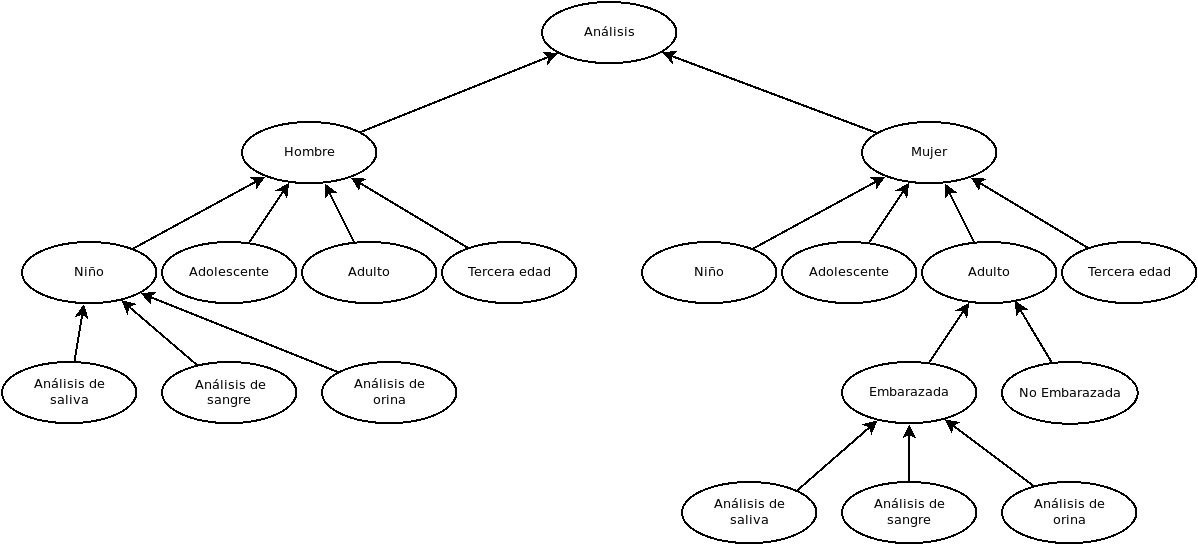
\includegraphics[width=\textwidth]{img/analisis.png}
	\caption{Diagrama de clases de análisis.}
	\label{fig:diagramaanalisis}
\end{figure}
\paragraph{}
Para poder representar todas las restricciones de dominio que presentan los análisis, tendremos que efectuar restricciones de dominio de la información tanto en sexo, como edad y tipo de análisis.
\paragraph{}
A esto le tenemos que añadir, en el caso de la mujer, el posible estado de embarazo a partir de la adolescencia.
\subsection{Atributos de los análisis}
\begin{itemize}
	\item {\bf Análisis}: \underline{Numero de extracción}, Fecha de la extracción, Umbrales de normalidad, Valores obtenidos, paciente, doctor, analistas, observaciones(*)
\end{itemize}

\paragraph{}
El analista deberá de tener acceso a una serie de factores modificadores de los resultados del análisis como los citados anteriormente en la sección
\ref{section:factoresatenerencuenta} (\nameref{section:factoresatenerencuenta}), estos serán almacenados como observaciones para su posterior uso por parte del personal cualificado.
\vfill
\begin{flushright}
	
	\small
	(*) Se refiere a los atributos no contemplados por los diagramas de la seción \ref{section:factoresatenerencuenta}
\end{flushright}

\pagebreak
\subsection{Restricciones de dominio de la información.}
\subsubsection{Restricciones de dominio según el sexo.}
\paragraph{}
Podemos diferenciar entre sexos ya que los umbrales de normalidad en los análisis pueden ser distintos en cada sexo.

\subsubsection{Restricciones de dominio según la edad.}
\paragraph{}
Debido a los diferentes rangos de valores aceptables en las distintas franjas de edades, haremos una distinción entre los distintos grupos de edades diferentes. Una posible clasificación sería la siguiente:
\begin{table}[hbt]
		\begin{center}
		\begin{tabular}{|c|c|}\hline
			subclase & franja de edad \\ \hline
			Niño & $<$10 \\ \hline
			Adolescente & 10-25 \\ \hline
			Adulto & 25-70 \\ \hline
			Tercera edad & $>$70 \\ \hline
		\end{tabular}
		\caption{Restricciones de dominio según la edad}
	\end{center}
\end{table}
\subsubsection{Restricciones de dominio según la naturaleza del análisis}
\paragraph{}
Según la naturaleza del análisis podemos distinguir entre varios tipos, en este ejemplo se consideran tres tipos de analíticas:
\begin{itemize}
	\item Análisis de sangre
	\item Análisis de saliva
	\item Análisis de orina
\end{itemize}
\subsubsection{Restricciones de dominio según el embarazo.}
\paragraph{}
En el caso de la mujer adolescente o la mujer adulta, habrá un nivel extra de especialización, uno para el estado no embarazada y otro para el estado embarazada. La entidad análisis se especificará en uno u otro dependiendo del estado de la mujer en el momento del análisis, ya que éste afectará en gran medida a muchos umbrales de normalidad.
\pagebreak
\subsection{Consideraciones según la normalidad del análisis}
\paragraph{}
En lo que respecta a la normalidad del análisis, estos podrán ser clasificados como $"$normales$"$ o $"$anómalos$"$.
\paragraph{}
Las mediciones normales son todas aquellas cuyos valores se encuentran en el umbral de aceptación de la subclase a la que instancian, si esto es cierto para todos los valores del susodicho análisis, éste sera considerado como normal.
\paragraph{}
En el caso de que una o varias mediciones se salgan del umbral de aceptación de dicha subclase, éste será clasificado como $"$Análisis Anómalo$"$.
\paragraph{}
Los umbrales serán definidos por un especialista en la materia debido a su alta complejidad.
\paragraph{}
Si el análisis es clasificado como anómalo, éste será marcado como tal en un sitio visible del impreso.
\paragraph{}
Además, antes de la impresión, se evaluará si la medición está entre los parámetros máximos y mínimos, si no lo está, la medición se marcará en un color distinto al del texto normal.
\paragraph{}
Nótese que solo el sexo, edad, y en el caso de la mujer, si esta está embarazada se han tenido en cuenta para los máximos y los mínimos. El resto de factores se almacenarán en el atributo $"$observaciones$"$ en las instancias de las subclases correspondientes al tipo de análisis, para su posterior consideración por el personal cualificado.
\pagebreak

\section{Diagrama de clases de personas.}
\paragraph{}
En el análisis participan tres agentes: el paciente al que se realiza el análisis, el doctor que receta el análisis y el analista que lleva a cabo el análisis en el laboratorio.
\paragraph{}
El diagrama de abstracción sería el siguiente:
\vspace{0.5cm}
\begin{center}
	\begin{figure}[hbt]
		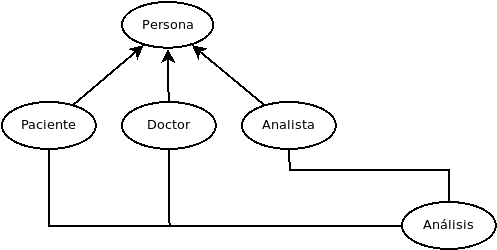
\includegraphics[width=\textwidth]{img/personas.png}
		\caption{Diagrama de clases de personas.}
		\label{fig:diagramapersonas}
	\end{figure}
\end{center}
\paragraph{}
Para que un análisis sea realizado éste debe ser mandado por un médico salvo en algunos casos excepcionales.
\subsection{Atributos de las personas}

\paragraph{}
Los atributos que se guardarán de las distintas clases serán los siguientes:
\begin{itemize}
	\item {\bf Paciente}: \underline{Número de la Seguridad Social}, historial cliínico, sexo, fecha de nacimiento y lugar de nacimiento.
	\item {\bf Doctor}: \underline{Número de colegiado} y campo o especialidad.
	\item {\bf Analista}: \underline{dni}, campo o especialidad y especialidad como analista.
\end{itemize}
\pagebreak
\subsection{Restricciones de dominio de la información}

\paragraph{}
Tanto los doctores como los analistas tendrán estar acreditados con las titulaciones correspondientes a la tarea desempeñada.
\paragraph{}
Las claves principales están marcadas con subrayado en los atributos de las clases Paciente, Doctor y Analista
\paragraph{}
Cada análisis tiene un id único (número de análisis), éste es generado automáticamente y es incremental, además, el análisis guarda de quién es (paciente), quién lo ha realizado (analista) y quien lo ha encargado (el doctor).
\subsection{Relaciones Persona-Análisis}
\paragraph{}
Referenciando a la figura ~\ref{fig:diagramaanalisis}, y figura ~\ref{fig:diagramapersonas} la multiplicidad de la relación entre análisis y las diferentes especializaciones de la entidad persona, son las siguientes:
\paragraph{Paciente-Análisis}
Debido a que un paciente podrá efectuar múltiples análisis, la relación sera de 1:N, ya que un análisis será solo de un cliente.
\paragraph{Doctor-Análisis}
De igual manera que la relación Paciente-Análisis, esta re-
lación tiene la multiplicidad 1:N, ya que un análisis solo puede como máximo
ser recetado por un doctor, pero en ciertos escenarios, no hace falta un doctor
que lo recete.

\paragraph{Analista-Análisis}
 Con multiplicidad N:N, ya que un análisis puede ser lle-
vado a cabo por varios analistas.

\pagebreak
\section{Consideraciones sobre Máquinas.}
En el laboratorio existen varios tipos de máquinas que pueden escribir o leer información de un análisis automáticamente:
% \vspace{0.5cm}\\
% 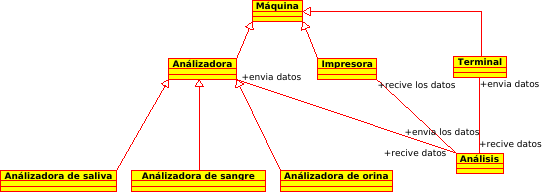
\includegraphics[width=\textwidth]{img/maquinas.png}
\paragraph{}
Como se puede observar, dentro de la entidad máquina, se encuentran los distintos tipos de máqinas que existen en el dominio del problema, en nuestro ejemplo hay tres tipos:
\begin{itemize}
	\item {\bf Analizadora}: Máquina encargada de obtener automáticamente los análisis de las muestras del paciente, a su vez, ésta se especializa en tres subclases, una por cada tipo de análisis en nuestro ejemplo:
	\begin{itemize}
		\item {\it Analizadora de sangre}.
		\item {\it Analizadora de saliva}.
		\item {\it Analizadora de orina}.
	\end{itemize}
	Estas máquinas pueden obtener ciertos resultados por ellas mismas sin intervención humana mas allá del posicionamiento de las muestras.
	\item {\bf Servicio de impresión}: Encargada de procesar e imprimir todo documento que se le mande.
	\item {\bf Terminal}: Debido a que no todas las mediciones podrán hacerse automáticamente por las máquinas, algunas muestras tendrán que ser analizadas por los analistas, éstos entonces podrán introducir los resultados a través de una terminal en el laboratorio.
\end{itemize}
\paragraph{}
Una vez completado el análisis, se mandará un documento generado a partir de los datos del análisis al servicio de impresión para su posterior recogida por el doctor que lo encargo.\\

% \pagebreak
% \section{Vista general.}
% \paragraph{}
% Gran parte del diagrama de análisis ha sido omitido.\\
% \vspace{0.7cm}\\
% 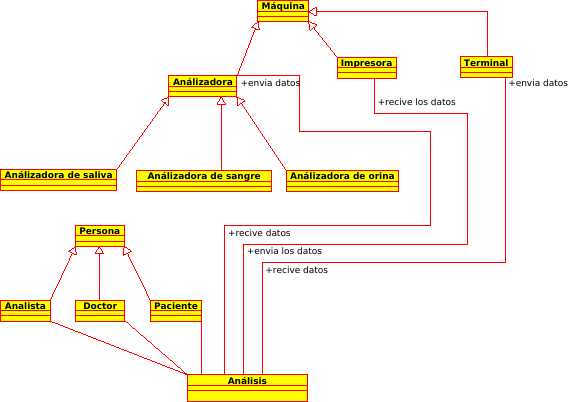
\includegraphics[width=\textwidth]{img/all.png}




%%%%%%%%%%%%%%%%%%%%%%%%%%%%%%%%%%%%%%%%%%%%%%%%%%%%%%%%%%%%%%%%%%%%%%%%%%%%%%%%
%%%%%%%%%%%%%%%%%%%%%%%%%%%%%%%%%%%%%%%%%%%%%%%%%%%%%%%%%%%%%%%%%%%%%%%%%%%%%%%%
%                           commented out things
%%%%%%%%%%%%%%%%%%%%%%%%%%%%%%%%%%%%%%%%%%%%%%%%%%%%%%%%%%%%%%%%%%%%%%%%%%%%%%%%
%%%%%%%%%%%%%%%%%%%%%%%%%%%%%%%%%%%%%%%%%%%%%%%%%%%%%%%%%%%%%%%%%%%%%%%%%%%%%%%%




% \section{Tabla de valores aceptables}
% \subsection{Análisis de sangre}
% \begin{center}
% 	\begin{tabular}{|c|c|c|c|c|c|c|c|c|c|} \hline
%
% 		% header
%
% 		\multirow{2}{*}{medida} & \multicolumn{4}{|c|}{Hombre} & \multicolumn{4}{|c|}{Mujer} & \multirow{2}{*}{unidades} \\ \cline{2-9}
% 		& 0-10 & 10-20 & 20-50 & 50+ & 0-10 & 10-20 & 20-50 & 50+ & \\ \hline
%
% 		% data
%
% %Glucosa,
%
% Glucosa & 100-180 & \multicolumn{3}{|c|}{90-130} & 100-180 &  \multicolumn{3}{|c|}{90-130} & mg/dL \\ \hline
% Colesterol total & \multicolumn{2}{c|}{$<$170} & \multicolumn{2}{c|}{125-200} &\multicolumn{2}{c|}{$<$170} & \multicolumn{2}{c|}{125-200} & mg/dL\\ \hline
% Colesterol HDL  &\multicolumn{4}{c|}{$<$100} &\multicolumn{4}{c|}{$<$100} & mg/dL\\ \hline
% Triglicéridos &  &  &  &  &  &  & & & \\ \hline
% Ácido úrico &  &  &  &  &  &  & & & \\ \hline
% Transaminasas &  &  &  &  &  &  & & & \\ \hline
% GOT/ASAT &  &  &  &  &  &  & & & \\ \hline
% GPT/ALT &  &  &  &  &  &  & & & \\ \hline
% Proteínas totales &  &  &  &  &  &  & & & \\ \hline
% Albúmina &  &  &  &  &  &  & & & \\ \hline
% Bilirrubina total &  &  &  &  &  &  & & & \\ \hline
% Hematíes (eritrocitos) &  &  &  &  &  &  & & & \\ \hline
% Hemoglobina &  &  &  &  &  &  & & & \\ \hline
% Hematocrito &  &  &  &  &  &  & & & \\ \hline
% V.C.M. &  &  &  &  &  &  & & & \\ \hline
% H.C.M. &  &  &  &  &  &  & & & \\ \hline
% C.H.C.M. &  &  &  &  &  &  & & & \\ \hline
% Leucocitos &  &  &  &  &  &  & & & \\ \hline
% Neutrófilos &  &  &  &  &  &  & & & \\ \hline
% Linfocitos &  &  &  &  &  &  & & & \\ \hline
% Monocitos &  &  &  &  &  &  & & & \\ \hline
% Eosinófilos &  &  &  &  &  &  & & & \\ \hline
% Basófilos &  &  &  &  &  &  & & & \\ \hline
% Hierro &  &  &  &  &  &  & & & \\ \hline
% Ferritina &  &  &  &  &  &  & & & \\ \hline
% Plaquetas &  &  &  &  &  &  & & & \\ \hline
% V.S.G. &  &  &  &  &  &  & & & \\ \hline
% Fibrinógeno &  &  &  &  &  &  & & & \\ \hline
%
%
% 	\end{tabular}
% \end{center}


% \raggedleft Document written in \LaTeX{}
\end{document}
